\documentclass[tikz,border=20pt]{standalone}
\usepackage{amsmath, amssymb}
\usetikzlibrary{positioning, arrows.meta, backgrounds, fit}

% Macros from your text
\newcommand{\Z}{\mathbb{Z}}
\newcommand{\C}{\mathbb{C}}
\newcommand{\F}{\mathbb{F}}
\newcommand{\ideal}[1]{\langle #1 \rangle}
\newcommand{\Spec}{\operatorname{Spec}}
\newcommand{\im}{\operatorname{im}}
\newcommand{\Ker}{\operatorname{Ker}}
\newcommand{\ol}[1]{\overline{#1}}

\begin{document}
	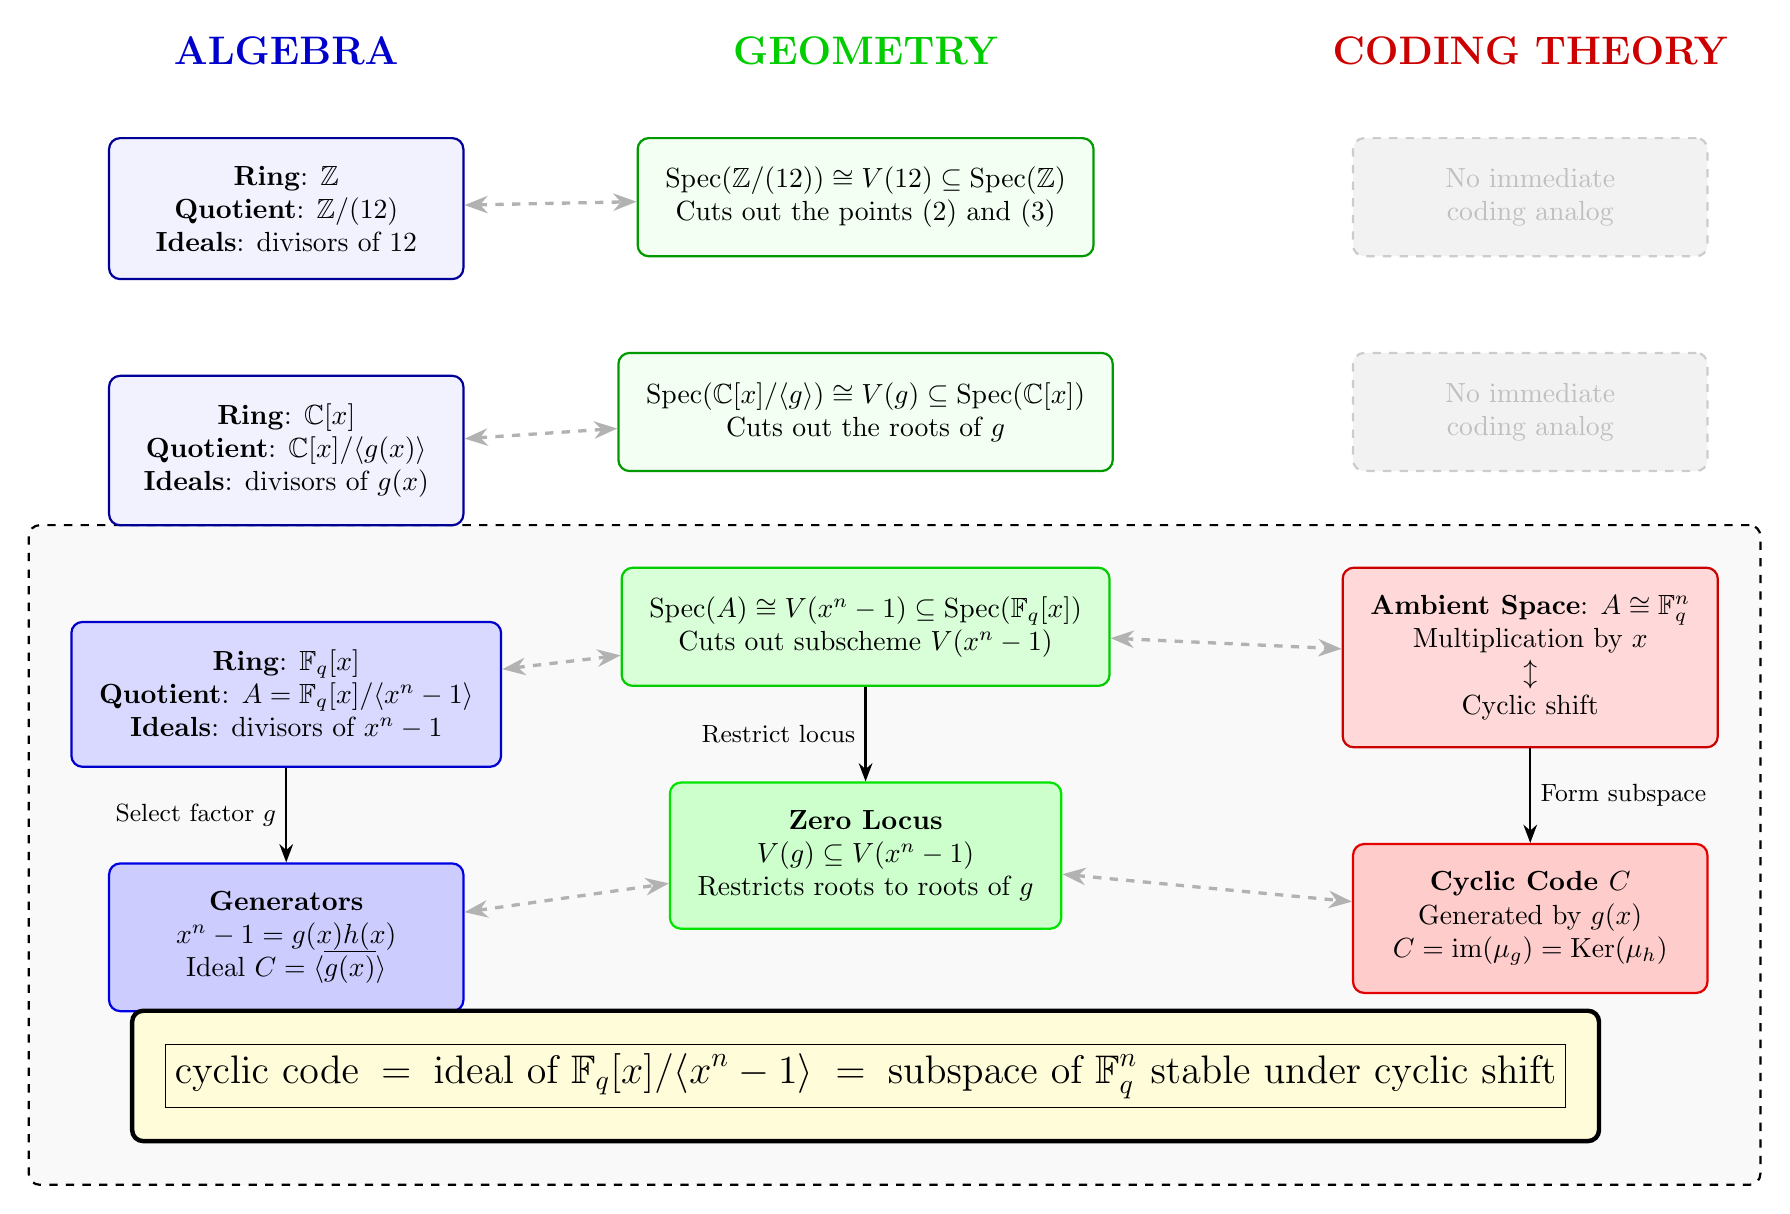
\begin{tikzpicture}[
		node distance=1.2cm and 1.5cm,
		box/.style={draw, thick, rounded corners, align=center, inner sep=10pt, minimum width=4.5cm, minimum height=1.5cm},
		alg/.style={box, fill=blue!5, draw=blue!60!black},
		geo/.style={box, fill=green!5, draw=green!60!black},
		cod/.style={box, fill=red!5, draw=red!60!black},
		na/.style={box, fill=gray!10, draw=gray!40, text=gray!50, dashed},
		arrow/.style={->, >=Stealth, thick},
		biarrow/.style={<->, >=Stealth, very thick, dashed, color=gray!60}
		]
		
		% ==========================================
		% COLUMN HEADERS
		% ==========================================
		\node[font=\Large\bfseries, color=blue!80!black] (h_alg) {ALGEBRA};
		\node[font=\Large\bfseries, color=green!80!black, right=4cm of h_alg] (h_geo) {GEOMETRY};
		\node[font=\Large\bfseries, color=red!80!black, right=4cm of h_geo] (h_cod) {CODING THEORY};
		
		% ==========================================
		% ROW 1: Arithmetic
		% ==========================================
		\node[alg, below=0.8cm of h_alg] (a1) {
			\textbf{Ring}: $\Z$ \\ 
			\textbf{Quotient}: $\Z/(12)$ \\ 
			\textbf{Ideals}: divisors of 12
		};
		\node[geo, below=0.8cm of h_geo] (g1) {
			$\Spec(\Z/(12)) \cong V(12) \subseteq \Spec(\Z)$ \\ 
			Cuts out the points $(2)$ and $(3)$
		};
		\node[na, below=0.8cm of h_cod] (c1) {
			No immediate \\ coding analog
		};
		
		\draw[biarrow] (a1) -- (g1);
		
		% ==========================================
		% ROW 2: Continuous / Complex
		% ==========================================
		\node[alg, below=of a1] (a2) {
			\textbf{Ring}: $\C[x]$ \\ 
			\textbf{Quotient}: $\C[x]/\ideal{g(x)}$ \\ 
			\textbf{Ideals}: divisors of $g(x)$
		};
		\node[geo, below=of g1] (g2) {
			$\Spec(\C[x]/\ideal{g}) \cong V(g) \subseteq \Spec(\C[x])$ \\ 
			Cuts out the roots of $g$
		};
		\node[na, below=of c1] (c2) {
			No immediate \\ coding analog
		};
		
		\draw[biarrow] (a2) -- (g2);
		
		% ==========================================
		% ROW 3: Finite Fields (The Intersection)
		% ==========================================
		\node[alg, below=of a2, fill=blue!15, draw=blue!80!black] (a3) {
			\textbf{Ring}: $\F_q[x]$ \\ 
			\textbf{Quotient}: $A = \F_q[x]/\ideal{x^n-1}$ \\ 
			\textbf{Ideals}: divisors of $x^n-1$
		};
		\node[geo, below=of g2, fill=green!15, draw=green!80!black] (g3) {
			$\Spec(A) \cong V(x^n-1) \subseteq \Spec(\F_q[x])$ \\ 
			Cuts out subscheme $V(x^n-1)$
		};
		\node[cod, below=of c2, fill=red!15, draw=red!80!black] (c3) {
			\textbf{Ambient Space}: $A \cong \F_q^n$ \\ 
			Multiplication by $x$ \\ $\updownarrow$ \\ Cyclic shift
		};
		
		\draw[biarrow] (a3) -- (g3);
		\draw[biarrow] (g3) -- (c3);
		
		% ==========================================
		% ROW 4: The Code Generation Mechanism
		% ==========================================
		\node[alg, below=of a3, fill=blue!20, draw=blue!90!black] (a4) {
			\textbf{Generators} \\ 
			$x^n-1 = g(x)h(x)$ \\ 
			Ideal $C = \ideal{\ol{g(x)}}$
		};
		\node[geo, below=of g3, fill=green!20, draw=green!90!black] (g4) {
			\textbf{Zero Locus} \\ 
			$V(g) \subseteq V(x^n-1)$ \\ 
			Restricts roots to roots of $g$
		};
		\node[cod, below=of c3, fill=red!20, draw=red!90!black] (c4) {
			\textbf{Cyclic Code $C$} \\ 
			Generated by $g(x)$ \\ 
			$C = \im(\mu_g) = \Ker(\mu_h)$
		};
		
		\draw[biarrow] (a4) -- (g4);
		\draw[biarrow] (g4) -- (c4);
		
		% Vertical progression arrows
		\draw[arrow] (a3) -- (a4) node[midway, left, font=\small] {Select factor $g$};
		\draw[arrow] (g3) -- (g4) node[midway, left, font=\small] {Restrict locus};
		\draw[arrow] (c3) -- (c4) node[midway, right, font=\small] {Form subspace};
		
		% ==========================================
		% BOTTOM: The Unified Boxed Equation
		% ==========================================
		\node[draw=black, ultra thick, rounded corners, fill=yellow!15, below=1cm of g4, minimum width=14cm, inner sep=12pt] (bottom_eq) {
			\Large $\boxed{
				\text{cyclic code}
				\;=\;
				\text{ideal of }\F_q[x]/\ideal{x^n-1}
				\;=\;
				\text{subspace of }\F_q^n\text{ stable under cyclic shift}
			}$
		};
		
		% ==========================================
		% BACKGROUND: Grouping the Rosetta Stone
		% ==========================================
		\begin{scope}[on background layer]
			% Draw a background box around the Finite/Code section to highlight the unification
			\node[draw, dashed, thick, rounded corners, fill=gray!5, inner sep=15pt, fit=(a3)(g3)(c3)(a4)(g4)(c4)(bottom_eq)] (highlight) {};
%			\node[above left, font=\bfseries\color=gray!60!black, xshift=-10pt, yshift=10pt] at (highlight.north east) {The Rosetta Stone Connection};
		\end{scope}
		
	\end{tikzpicture}
\end{document}